\documentclass{beamer}
\usetheme{metropolis} % Use metropolis theme





\title{ECON 3818: Introduction to Statistics with Computer Applications}
%\subtitle
\date{\today}
\author{Kyle Butts}



\definecolor{blue}{RGB}{0,114,178}

\definecolor{red}{HTML}{EB0E09}
\definecolor{yellow}{RGB}{240,228,66}
\definecolor{green}{RGB}{0,158,115}
\definecolor{maroon}{HTML}{AF3335}
\definecolor{purple}{HTML}{7E90B8}


\definecolor{mybackground}{HTML}{ECECEC}
\setbeamercolor{background canvas}{bg= mybackground}

\definecolor{buff-gold}{HTML}{CFB87C}
\definecolor{buff-grey}{HTML}{565A5C}
\definecolor{buff-lightgrey}{HTML}{A2A4A3}
\definecolor{buff-black}{HTML}{000000}

\setbeamercolor{alerted text}{fg=buff-gold!80!black}
\setbeamercolor{frametitle}{bg=buff-black}
\setbeamercolor{title}{fg=buff-grey}
\setbeamercolor{button}{bg=buff-gold}

% Allow to remove indent w/ \begin{itemize}[leftmargin= *]
\usepackage{enumitem}
\setlist[itemize]{label= \textbullet}

% \usepackage[libertine]{newtxmath}
\usepackage{longtable}
\usepackage{booktabs}
\usepackage{enumitem}







\begin{document}

% Title Page ---------------------------------------
\maketitle




% Chapter 16 ---------------------------------------
\section{Chapter 16: Confidence Intervals}
\begin{frame}{Statistical Inference}
	
	Recall, we're interested in estimating some unknown population parameter $\theta$ using the sample $X_1, ...,X_n$
	\begin{itemize}
		\item We can use some estimator $\hat{\theta}$
		      \begin{itemize}
		      	\item We can find its bias and its variance
		      	\item Can say what it converges to using LLN and CLT
		      \end{itemize}
		\item There are limitations of estimation process
		      \begin{itemize}
		      	\item Using $\bar{X}$ to estimate $\mu$, but since $\bar{X} \sim N(\mu, \frac{\sigma^2}{n})$, and the normal distribution is a continuous distribution, $P(\bar{X}=\mu)=0$
		      \end{itemize}
	\end{itemize}
	Therefore we need to construct some belief about how good our estimator is
	
\end{frame}


%\begin{frame}{Introduction}
%Lets begin by exploiting what we know about probability distributions of sample statistics 
%\begin{itemize}
%\item Example: $\bar{X}$ calculated from a SRS normally distributed population
%$$P(\mu - k<\bar{X}<\mu + k)=0.95$$
%%%put picture in (or draw on the board)
%\end{itemize}
%\end{frame}


\begin{frame}{Example}
	\small{Say we collect BMI measures for 654 women, and calculate $\bar{X}=26.8$. Somehow we also know that $\sigma$=7.5

	\pause
	\vskip.2in
	The 95 part of the 68-95-99.7 rule for Normal distributions says that $\bar{X}$ is within 2 standard deviations of the mean $\mu$ in 95\% of samples. 
	\vskip.2in
	
	\pause
	Since $\sigma=7.5$, the std deviation of $\bar{X}=\frac{7.5}{\sqrt{654}}=0.3$. This means 95\% of all samples of size 654, the distance between the sample mean $\bar{X}$ and the population mean $\mu$ is less than 0.6 (two std deviations).
	\vskip.2in

	\pause
	So if we estimate that $\mu$ lies somewhere in the interval from $\bar{X}-0.6$ to $\bar{X}+0.6$, we'll be right for 95\% of all possible samples.}
\end{frame}


\begin{frame}{Confidence Intervals}
	\begin{center}
		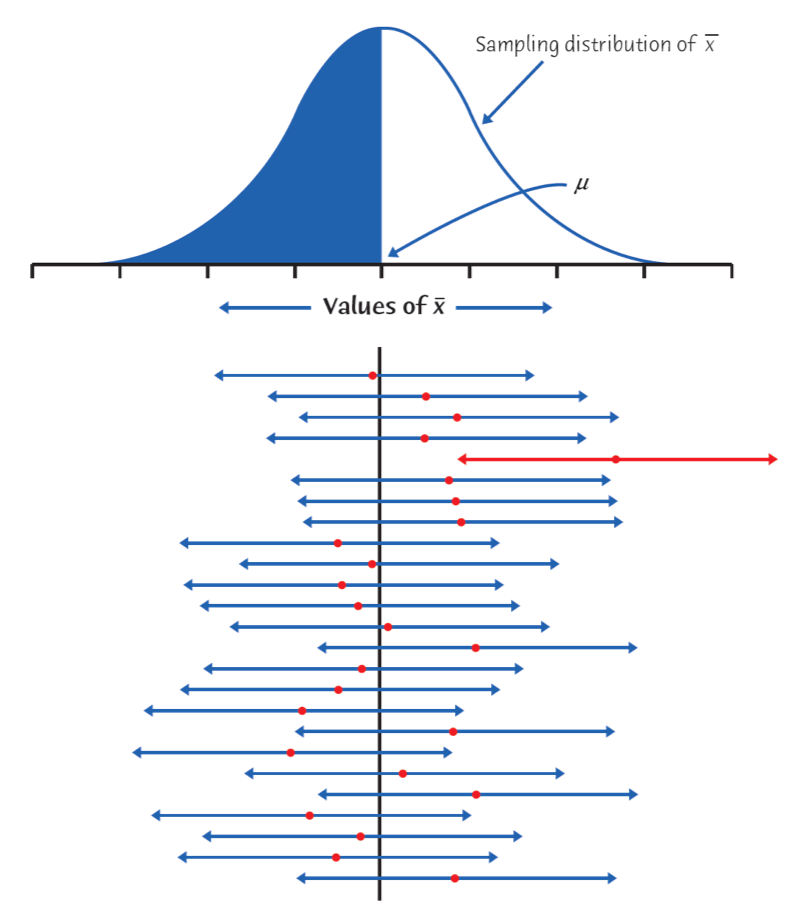
\includegraphics[width=0.6\textwidth]{repeatedci}
	\end{center}
\end{frame}

\begin{frame}{Introduction}
	Plugging in all the information we have leads to:
	\vskip.2in
	$$\big[26.8-0.6, 26.8+0.6\big] = \big[ 26.2, 27.4 \big]$$
	\vskip.4in
	This interval is a \alert{confidence interval}, which says that we are  \textit{95\% confident} that the true mean of the BMI, $\mu$, is in between 26.2 and 27.4

	\pause
	\begin{itemize}
		\item \textbf{This is because we got this interval from a method that captures the population mean for 95\% of all possible samples}
	\end{itemize}
\end{frame}

\begin{frame}{Confidence Intervals}
	In that example, the confidence interval was $\bar{X} \pm 0.6$. In general, a confidence interval takes the form 
	$$\text{ estimate } \pm \text{ margin of error }$$
	where the \alert{margin of error} shows how much variability there is in our estimate
\end{frame}

\begin{frame}{Margins of Error}
	We define the margin of error for our sample mean as: \[
		k=Z_{\frac{1-C}{2}} \frac{\sigma}{\sqrt{n}},
	\]

	where C is our level of confidence
	
	\begin{itemize}
		\item 90\% Confidence Interval $\rightarrow Z_{\frac{1-C}{2}} = Z_{.05} = 1.645$ 
		
		\item We want to split the remaining 10\% across the two tails, so we calculate the z-score that gives us 5\% to the right, which is 1.645
	\end{itemize}
\end{frame}

\begin{frame}{Example}
	Lets determine the \textit{exact} margin of error for previous example
	$$k=Z_{\frac{1-C}{2}} \cdot \frac{\sigma}{\sqrt{n}}$$
	
	
	If we are calculating 95\% confidence interval, where $\bar{X}_{654}=26.8$ $\sigma = 7.5$,  then
	$$k=Z_{0.025} \cdot \frac{7.5}{\sqrt{654}}$$
	\vskip.2in
	We find $Z_{0.025}$ using the table. $Z_{0.025}$ is the z-score such that $P(Z>Z_{0.025})=0.025$
\end{frame}

\begin{frame}{Example}
	Using the z-table, we find that $Z_{0.025} = 1.96$. This means:
	$$k=1.96\cdot \frac{7.5}{\sqrt{654}}=0.57$$
	\vskip.5in
	This means our \textit{exact} 95\% confidence interval is:
	$$[26.23, 27.37]$$
\end{frame}

\begin{frame}{Clicker Question}
	What Z-score will be associated with a 82\% confidence interval
	
	\begin{enumerate}[label=(\alph*)]
		\item 0.92
		\item 1.34 %
		\item 0.82
		\item 0.79
	\end{enumerate}
\end{frame}

\begin{frame}{Clicker Question}
	A 95\% confidence interval for the mean hours freshmen spent on social media per day was calculated to be [2.5 hours, 3.1 hours] based off a sample mean $\bar{X}=2.8$. The confidence interval was based on a SRS sample of n=50. The standard deviation is given by:
	
	\begin{enumerate}[label=(\alph*)]
		\item 0.3
		\item 1.96
		\item 0.2772
		\item 1.0823
	\end{enumerate}
\end{frame}

\begin{frame}{Margins of Error}
	So to recap, the margin of error is calculated by:
	$$k=Z_{\frac{1-C}{2}} \cdot \frac{\sigma}{\sqrt{n}}$$
	\vskip.2in
	This means the size of the margin of error is determined by:
	\begin{itemize}
		\item level of confidence
		\item size of sample (can sometimes control)
		\item variance (which we can't control)
	\end{itemize}
\end{frame}


\begin{frame}{Clicker Question}
	Given a sample mean of 8, from a sample of 36 observations, and a variance of 25, construct 90\%, 95\%, and 99\% confidence intervals for the true value, $\mu$. Rank the intervals from largest to smallest:
	\begin{enumerate}[label=(\alph*)]
		\item 99\%, 95\%, 90\%
		\item 90\%, 95\%, 99\%
		\item They're all the same size
	\end{enumerate}
\end{frame}

\begin{frame}{Margins of Error}
	As we've mentioned, the margin of error is determined by: 
	\begin{itemize}
		\item Level of confidence
		      \begin{itemize}
		      	\item higher the level of confidence we want to have, larger the margin of error
		      \end{itemize}
		\item Size of sample 
		      \begin{itemize}
		      	\item larger the sample, smaller the margin of error
		      \end{itemize}
		\item Variance
		      \begin{itemize}
		      	\item larger the variance, larger the margin of error
		      \end{itemize}
	\end{itemize}
\end{frame}

\begin{frame}{Confidence Intervals}
	How to think of a confidence interval:
	
	\begin{itemize}
		\item You collect many different samples from the population
		\item For each sample, you calculate the mean and the associated confidence interval around that mean
		\item You'll have a confidence interval for each sample you collected
		\item \textbf{95\% of the confidence intervals you calculated will include the true mean $\mu$}
	\end{itemize}
\end{frame}

\begin{frame}{Confidence Intervals}
	Common misconceptions about confidence intervals
	\begin{itemize}
		\item The CI \alert{does not} tell you:
		      \begin{itemize}
		      	\item The true mean is inside the confidence interval
		      	\item The true mean is \alert{certainly} inside your CI, C\% of the time
		      	\item The probability the true mean is in your CI is  C\%
		      \end{itemize}
		      \vskip.2in
		\item The CI \alert{does} tell you:
		      \begin{itemize}
		      	\item the range of estimates that contain the true mean  C\% of the time \alert{in repeated sampling}
		      \end{itemize}
	\end{itemize}
\end{frame}

\begin{frame}{Clicker Question -- Midterm Example}
	Veterinary researchers at a major university veterinary hospital calculated a 99\% confidence interval for the average age of horses admitted for laminitis (a particular foot disease) as 6.3 to 7.4 years. Based on this information we conclude that:
	
	\begin{enumerate}[label=(\alph*)]
		\item 99\% of all horses admitted for laminitis are between 6.3 and 7.4 years old
		\item 99\% of the time, the average age of a horse admitted for laminitis will be between 6.3 and 7.4 years
		\item We are 99\% confident that the true mean age of horses with laminitis is between 6.3 and 7.4 years old
		\item 99\% of all samples of size n=25 will have an average age of horses with laminitis between 6.3 and 7.4 years old.
	\end{enumerate}
\end{frame}



\begin{frame}{Confidence Intervals}
	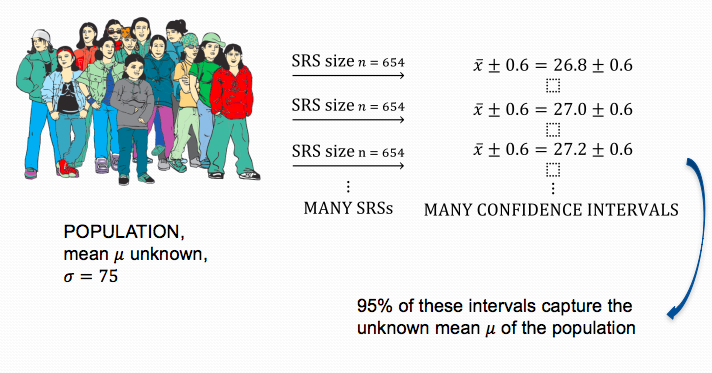
\includegraphics[width=\textwidth]{ci_pic}
\end{frame}

\begin{frame}{Confidence Intervals}
	\begin{center}
		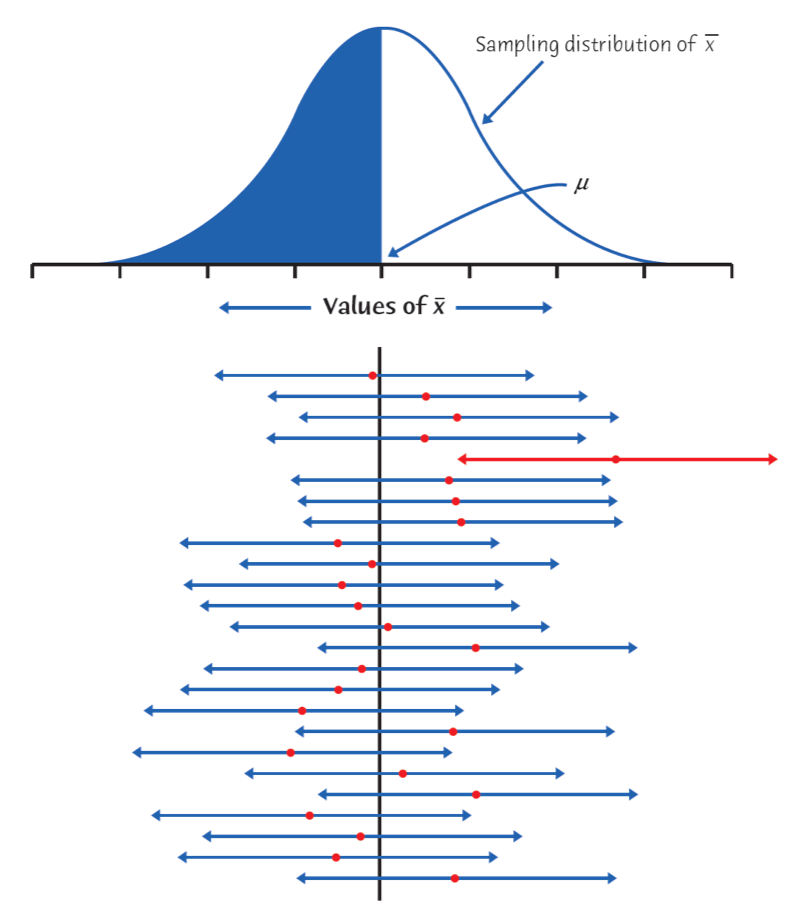
\includegraphics[width=0.6\textwidth]{repeatedci}
	\end{center}
\end{frame}









\end{document}